\documentclass[12pt]{article}


\usepackage{latexsym}
\usepackage[margin=1in]{geometry}
\usepackage{graphicx}
\usepackage{subfig}
\usepackage{enumerate}
\usepackage{multirow}
\usepackage{booktabs}
%\usepackage{mathptmx}
\usepackage[square]{natbib}
\usepackage{amsmath}
\usepackage{amsfonts}
\usepackage{amssymb}
\usepackage{amsbsy}
\usepackage{amsthm}
\usepackage[pdftex,colorlinks=true,urlcolor=blue,citecolor=black,anchorcolor=black,linkcolor=black]{hyperref}
\usepackage{setspace}

\onehalfspacing

\newtheorem{theorem}{Theorem}
\renewcommand{\thetheorem}{ \arabic{theorem}}
\newtheorem{corollary}[theorem]{Corollary}
\renewcommand{\thecorollary}{\arabic{corollary}}
\newtheorem{definition}{Definition}
\renewcommand{\thedefinition}{\arabic{definition}}
\newtheorem{lemma}{Lemma}
\renewcommand{\thelemma}{ \arabic{lemma}}
\newtheorem{proposition}{Proposition}
\renewcommand{\theproposition}{ \arabic{proposition}}
\newtheorem{remark}{Remark}
\renewcommand{\theremark}{ \arabic{remark}}

% Frequently used general mathematics
\newcommand{\R}{{\mathbb{R}}}
\newcommand{\Rp}{\R^+}
\newcommand{\Z}{{\mathbb{Z}}}
\newcommand{\Zp}{\Z^+}
\newcommand{\Q}{\mathbb{Q}}
\newcommand{\N}{\mathbb{N}}

% Commands for probability
\newcommand{\p}[1]{\mathbb{P} \left\{ #1 \right\}}
\newcommand{\e}[1]{\mathbb{E} \left[ #1 \right]
}
\newcommand{\ee}[2]{\mathbb{E}_{#1} \left[ #2 \right]}
\newcommand{\var}[1]{\mathrm{Var} \left( #1 \right)}
\newcommand{\cov}[1]{\mathrm{Cov} \left( #1 \right)}
\newcommand{\cor}[1]{\mathrm{Corr} \left( #1 \right)}
\newcommand{\varh}[1]{\widehat{\mathrm{Var}} \left( #1 \right)}
\newcommand{\vart}[1]{\widetilde{\mathrm{Var}} \left( #1 \right)}
\newcommand{\vartg}[1]{\widetilde{\mathrm{Var}}_\gamma \left( #1 \right)}
\newcommand{\vto}[1]{\widetilde{\mathrm{Var}}_{1} \left( #1 \right)}
\newcommand{\vtm}[1]{\widetilde{\mathrm{Var}}_{m} \left( #1 \right)}
\newcommand{\varhat}{\widehat{\mathrm{Var}}}

% Definitions of variables
\newcommand{\X}{X}
\newcommand{\x}{\mathbf{x}}
\newcommand{\xh}{{\hat{\x}}}
\newcommand{\xs}{\x^*}
\newcommand{\xit}{\boldsymbol{\xi}}
\newcommand{\xiti}{\xit^i}
\newcommand{\zs}{z^*}
\newcommand{\nb}{\left\lfloor\tfrac{n-m}{\gamma}\right\rfloor+1}
\newcommand{\nbl}{\left\lfloor\tfrac{n_l-m_l}{\gamma_l}\right\rfloor+1}
\newcommand{\gammab}{\bar{\gamma}}
\newcommand{\ogb}{\tfrac{1}{\gammab}}
\newcommand{\cogb}{\left\lceil\ogb\right\rceil}

% Definitions for overlapping batches
\newcommand{\gb}{\bar{G}}
\newcommand{\gbb}{\bar{\gb}}
\newcommand{\db}{\bar{D}}
\newcommand{\dbb}{\bar{\db}}

% Used only for review of Meketon.
\newcommand{\y}{\mathbf{y}}
\newcommand{\yb}{\bar{y}}
\newcommand{\ybb}{\bar{\yb}}

\DeclareMathOperator*{\argmin}{argmin}

\newcommand{\Keywords}[1]{\par\noindent 
{\small{\em Keywords\/}: #1}}



%#########################################################
%*
%*  The Document.
%*
\begin{document}

\title{Overlapping Batches for the Assessment of Solution Quality in Stochastic Programs}

\author{David~Love$^{a}$\ \ and G\"{u}zin~Bayraksan$^{b}$\thanks{Corresponding author. Tel.: +1 614-292-1695. Fax:+1 614-292-7852}\\[6pt]
{\small
      $^{a}$ Program in Applied Mathematics, University of Arizona, Tucson, AZ 85721, USA,}\\
{\small \ \ \ \ \ \texttt{dlove@math.arizona.edu}} \\
{\small 
      $^{b}$ Integrated Systems Engineering, The Ohio State University, Columbus, OH 43210, USA,}\\
{\small \ \ \ \  \   \texttt{bayraksan.1@osu.edu}}}
\date{}

\maketitle

\begin{abstract}
\noindent Overlapping Batch Means (OBM) has long been used in simulation as a method of reusing data to generate variance estimators with asymptotically lower variance.
In this paper, we apply the OBM method to stochastic programming by formulating a variant of the multiple replications procedure used for assessing solution quality.
We give conditions under which the resulting optimality gap point estimators are strongly consistent, the optimality gap interval estimators are asymptotically valid, and the OBM variance estimators for optimality gap have asymptotically lower variances relative to their nonoverlapping counterparts \citep{Meketon1984,Welch1987}.
We investigate computational efficiency, a combined measure of variance and computation time, providing guidelines on the degree of overlap.  
Numerical experiments on several test problems are presented, examining the small-sample behavior and the empirical computational efficiency of the overlapping batches method in this context.  
\medskip

\Keywords{Sample average approximation (SAA); Overlapping batch means;   Stochastic programming; Optimality gap estimation}
\end{abstract}


%%%%%%%%%%%%%%%%%%%%%%%%%%%%%%%%%%%%%%%%%%%%%%%%%%%%%%%%%%%%%%%%%%%%%%%%%%%%%%%%
\section{Introduction}
\label{sec:intro}

The Overlapping Batch Means (OBM) method, proposed by \citet{Meketon1984}, is commonly used in simulation to obtain variance estimators having variances that are comparatively lower than their nonoverlapped counterparts. 
In the context of steady-state simulation, OBM is often used to estimate the variance of the sample mean, which is itself an estimator for the mean. 
\cite{SAH90} use overlapping estimators to estimate the variance of estimators for non-means. 
More recently, overlapping estimators based on standardized time series (as opposed to batch means) have been evaluated \citep{Alexopoulos01012007,Alexopoulos2007}; see also \cite{Meterelliyoz_etal_12}.
To the best of our knowledge, OBM has never before been studied in a stochastic optimization context. 
In this paper, we show that the overlapping batches achieve nearly the same bias and lower variances relative to their nonoverlapped counterparts when used in a stochastic optimization setting.
  
A natural setting where batch means are used in stochastic optimization (especially in stochastic programming) is for assessing solution quality. 
This typically involves generating point and interval estimators of the optimality gap of a given candidate solution using Monte Carlo simulation. 
Because optimality gap estimators can be difficult to analyze statistically, a common approach is to use nonoverlapping batches of data to generate a number of optimality gap estimators. 
These individual estimators are then used to form point and interval estimators applying the nonoverlapping batch means method.
This is referred to as the Multiple Replications Procedure (MRP) and was initially discussed in \cite{Mak1999}.   
In this paper, we formulate an overlapping batches version of MRP.


We consider a stochastic optimization problem of the form 
\begin{align} \tag{SP} \label{eq:sto_prog} 
	z^* & = \min_{\x \in X} \e{f(\x,\xit)},
\end{align}
where $\x$ is a vector of decision variables, $\xit$ is a vector of random variables, and $X$ is the feasible set, which consists of only deterministic constraints. 
We assume (\ref{eq:sto_prog}) has no stochastic constraints such as probabilistic or expected-value constraints. 
Further, it is assumed that the distribution of $\xit$ is known and that we can sample from it.
Even though we will impose a more-restrictive moment condition later, we assume that $\e{f(\x,\xit)}$ is well defined and finite for all $\x \in X$ and (\ref{eq:sto_prog}) has a finite optimal solution achieved on $X$.


Unless $f$ has a simple structure or the number of realizations of $\xit$ is small, (\ref{eq:sto_prog}) typically cannot be solved exactly. 
An approximation of (\ref{eq:sto_prog}) can be generated by sampling from the distribution of $\xit$.
While other sampling schemes are possible, let $\xit^1, \xit^2, \dots, \xit^m$ be an independent and identically distributed (i.i.d.) sample from the distribution of $\xit$.
A sampling approximation of (\ref{eq:sto_prog}), often called the sample average approximation, is given by\vspace*{-0.07in}
\begin{align} \tag{SP$_m$} \label{eq:sto_prog_m}
	z_m^* & = \min_{\x \in X} \frac{1}{m} \sum_{i=1}^m f(\x,\xiti).
\end{align}
We denote an optimal solution to (\ref{eq:sto_prog}) as $\xs$ and an optimal solution to (\ref{eq:sto_prog_m}) as $\xs_m$.



We wish to assess the quality of a candidate solution $\xh \in X$, which may have been found in any way.
Assessing solution quality is important in practice because as (\ref{eq:sto_prog}) typically cannot be solved exactly, one only has an approximate solution $\xh$ without verification of its quality.
Assessing solution quality is also a critical component of stopping criteria in algorithms designed to (approximately) solve (\ref{eq:sto_prog}).
We define the quality of $\xh$ by its optimality gap, $\e{f(\xh,\xit)} - \zs$. 
The lower the optimality gap, the higher the quality of the solution; and a zero optimality gap implies that the solution is optimal. 
We assume that the candidate solution $\xh$ is given as input to our procedures, and hence fixed, throughout the paper. 


The optimality gap $\e{f(\xh,\xit)} - \zs$ often cannot be calculated exactly. First, for a given candidate solution $\xh \in X$, evaluation of $\e{f(\xh,\xit)}$ typically involves a difficult multidimensional integral. 
Second, we do not know $\zs$. 
In many fields of optimization, the second problem is alleviated by obtaining lower bounds on $\zs$ through relaxations such as integrality, Lagrangian, or semidefinite relaxations.
As a result, it is common to evaluate an upper bound on the optimality gap. 
This motivates estimating the upper bound on the optimality gap in stochastic programming by using Monte Carlo simulation.
Given a sample size $m$, an upper bound on the optimality gap can be obtained by $$
\e{f(\xh,\xit)} - \zs \leq \e{f(\xh,\xit)} - \e{\zs_m}
$$ 
due to the inequality $\e{\zs_m} \leq \zs$ \citep{Mak1999,norkin_pflug_ruszczynski_98}.
This bound improves as the sample size increases; that is, $\e{\zs_m} \leq \e{\zs_{m+1}} \leq \zs$.  
A straightforward estimate of $\e{f(\xh,\xit)}$ is the sample mean, $\frac{1}{m} \sum_{i=1}^m f(\xh,\xiti)$. 
Instead of $\e{\zs_m}$, we can simply use $\zs_m$.  
The resulting point estimator of the optimality gap is then 
$$
\frac{1}{m} \sum_{i=1}^m f(\xh,\xiti) - \zs_m.
$$ 
Here, we assume the same observations $\xit^1, \dots, \xit^m$ are used in both terms.  

Computing the above optimality gap estimate involves solving the optimization problem (\ref{eq:sto_prog_m}) to obtain a lower bound estimator of $\zs$, $\zs_m$, which complicates the statistical analysis. 
As mentioned above, to enable statistical inference, the MRP of \citet{Mak1999} generates $k$ independent estimators, each using sample size $m$ ($k$ nonoverlapping batches of size $m$), and averages them to obtain a point estimator.  
The sample variance of these estimators is used to form confidence intervals (CIs) for the optimality gap (we further review MRP in \S \ref{ssec:mrp}).  
An advantage of MRP is its applicability to a wide range of problems.  
With i.i.d.\ sampling, $f$ can be linear or nonlinear, $\X$ can include integrality constraints or not.  
It is also easy to implement; thus, MRP has been applied to a wide variety of problems, including finance, supply chain network design, etc.; see, e.g., \cite{bertocchi_etal_99,janjarassuk_linderoth_08,santoso_ahmed_etal_05}.  
Recently, the approach of (nonoverlapping) batching has been used for assessing solution quality of stochastic programs with finitely many expected value \citep{wang_ahmed_08} and stochastic dominance \citep{hu2010sample} constraints.
 


Our aim is to apply the idea of overlapping batches to MRP.  
The motivation behind using overlapping batches in this context is twofold. 
First, overlapping could help to obtain better variance estimators with simple data reuse, resulting in improved CIs.
Second, in some cases, generating the realizations $\xit^1, \xit^2, \dots$ to form sampling approximations of (\ref{eq:sto_prog}) can be computationally expensive, and in these cases, overlapping makes the most of the generated observations by reusing data. 

The contributions of this article are as follows: 
\begin{itemize}
\item[(i)] We formulate an overlapping batch means variant of MRP, where the degree of overlap can be chosen by the user.  
This application of OBM is novel because each batch mean estimator includes an internal minimization, which has not been studied in the literature.
%\vspace*{-0.1in}

\item[(ii)] We provide conditions under which the resulting optimality gap estimators exhibit reduced variance when compared to their counterparts obtained via nonoverlapping batches.
We also show that the resulting point estimators are strongly consistent and that the interval estimators are asymptotically valid. 
These results require new proofs because of the presence of the optimization operator. 

\item[(iii)] We examine small-sample behavior of the estimators through numerical examples. 
Our experiments indicate that the use of overlapping estimators results in gap estimators achieving lower variance than their nonoverlapping counterparts, along with comparable bias and interval coverage---for both small- and large-sample cases.

\item[(iv)] As the degree of overlap increases, the number of batches---and optimization problems solved---increases because we need to solve a sampling problem per batch. 
At the same time, variances are lowered, and when warm starting is available, solution time per batch can decrease, yielding efficiency gains. 
We explore this trade-off between computation time and lower variances.
Our results indicate that when warm starting is effective, overlapping estimators are computationally more efficient than those formed via nonoverlapping batches.
Based on this study, we provide guidelines on selecting the degree of overlap and demonstrate efficiency on a newsvendor problem. 
\end{itemize}


An earlier version of the paper appeared in \cite{love2011overlapping}. 
Most of the theoretical results in the current version of the paper are new, including almost sure convergence and asymptotically lower variances of the overlapping variance estimators, and asymptotic validity of the interval estimators. 
These results are achieved through a stronger assumption on the rate of convergence of the sampling problem's solution to the unique optimal solution, which is satisfied by several classes of (\ref{eq:sto_prog}); see \S \ref{subsec:assumptions}.
We also present additional computational results, including those from a large-scale problem, and study computational efficiency of the overlapping MRP method. 



The rest of the paper is organized as follows.  
In the next section, we review relevant background information.  
We first discuss nonoverlapping and overlapping batch means in \S \ref{ssec:obm} and then briefly go over MRP in \S \ref{ssec:mrp}.  
In \S \ref{sec:omrp}, we present the Overlapping Multiple Replications Procedure (OMRP) with a parametrized degree of overlap.  
In \S \ref{sec:theory}, we show strong consistency of the OMRP point estimators, asymptotic validity of the OMRP CIs, and establish that the OMRP variance estimators have lower variances than their nonoverlapping MRP counterparts.
In \S \ref{sec:comp}, we test the performance of OMRP on four problems and study computational efficiency. 
We end in \S \ref{sec:concl} with a summary and conclusions.


%%%%%%%%%%%%%%%%%%%%%%%%%%%%%%%%%%%%%%%%%%%%%%%%%%%%%%%%%%%%%%%%%%%%%%%%%%%%%%%%
\section{Background}
\label{sec:background}


\subsection{Batch Means} 
\label{ssec:obm}

Consider a covariance stationary stochastic process $y^1, y^2, \dots$ with mean $\mu$ and variance parameter $0<\sigma^2<\infty$.  
The variance parameter is the sum of covariances at all lags, $\sigma^2=\mathrm{Var} \left(y^1 \right)+2\sum_{j=1}^{\infty}\mathrm{Cov} \left(y^1,y^{1+j}\right)$. 
If the variance parameter exists, then  $\sigma^2=\lim_{n\rightarrow \infty}n\mathrm{Var} \left(\ybb\right)$, where $\ybb=\frac{1}{n}\sum_{i=1}^{n} y^{i}$.
The task is to estimate $\mu$ given some realization of the univariate stochastic process $\y = (y^1, y^2, \dots, y^n)$.  
Typically, this involves forming a CI of the form $[L_\alpha(\y), U_\alpha(\y)]$ for a given level of significance $\alpha$ such that $\p{L_\alpha(\y) \leq \mu \leq U_\alpha(\y)} = 1 - \alpha$ or that this probability is approximately $1 - \alpha$ for large enough sample sizes.  
The usual estimator for $\mu$ is the sample mean $\ybb$, which is an unbiased estimator even in the presence of correlated data.  
However, the usual (sample) variance estimator $\frac{1}{n-1} \sum_{i=1}^n (y^i - \ybb)^2$ can be inappropriate to use in the presence of correlated data, resulting in inaccurate interval estimators.  
To overcome this difficulty, various variance estimators have been proposed in the simulation literature; see, e.g., \cite{law_15}.  
We briefly review two of these variance estimators: nonoverlapping and overlapping batch means.

\subsubsection{Nonoverlapping Batch Means}

Nonoverlapping batch means takes $n$ observations $y^1, \dots, y^n$ of the stochastic process and splits them into $k$ batches of size $m$, where $k = \frac{n}{m}$ (for simplicity, assume, for now, $n = mk$).  
In the application under consideration in this article, the observations {\it within} a batch are correlated due to the optimization in each batch; see \S \ref{ssec:mrp} for details. 
The sample mean of each batch is computed as
$
	\yb_j = \frac{1}{m} \sum_{i=1}^{m} y^{m(j-1)+i}, j = 1,2, \dots, k,
$
and the overall sample mean $\ybb = \frac{1}{k} \sum_{j=1}^k \yb_j = \frac{1}{n} \sum_{i=1}^n y^i$ provides a point estimator of $\mu$.  
The variance estimator of the batch means, which is $m/n$ times the sample variance, is calculated as
\begin{equation} \label{eq:var}
	\varhat(\ybb) = \frac{m}{n}\frac{1}{k-1} \sum_{j=1}^k \left( \yb_j - \ybb \right)^2.
\end{equation}
The $(1-\alpha)$-level approximate CI is then formed by $\ybb \pm t_{k-1,\alpha/2} \sqrt{\varhat(\ybb)}$, where $t_{k-1,\alpha/2}$ denotes the $1-\alpha/2$ quantile of the Student's t distribution with $k-1$ degrees of freedom.  
Under appropriate conditions, $n\varhat(\ybb)$ is a consistent estimator of $\sigma^2$ \citep{alexo_enc_06}.

\subsubsection{Overlapping Batch Means}
\label{ssec:overlap}

Overlapping batch means modifies nonoverlapping batch means by reusing a subset of observations from one batch to form the next batch. 
In this paper, we use the {\it batch nonoverlap parameter} $1 \leq \gamma \leq m$ to denote how much neighboring batches do {\it not} overlap.  
For instance, $\gamma = m$ corresponds to the case of nonoverlapping batches and $\gamma = 1$ corresponds to the maximally overlapping case of \citet{Meketon1984}.  
In general, $\gamma$ can take any integer value between and including $[1,m]$. 
Let $\lfloor \cdot \rfloor$ be the greatest integer that is less than or equal to its argument. 
The sample mean of each overlapping batch is calculated similarly, 
$
\yb_j = \frac{1}{m} \sum_{i=1}^m y^{\gamma(j-1) + i},\ \  j = 1, 2, \dots, \nb, 
$
now taking into account $\gamma$.  
Here, $\nb$ batches are formed given $n$, $m$, and $\gamma$.  
The variance estimator is updated to
\begin{equation} \label{eq:variance_gamma}
	\vartg{\ybb} = \frac{1}{\left( \tfrac{n}{m} - 1 \right) \left( \nb \right)}  \sum_{j=1}^{\nb} (\yb_j - \ybb)^2.
\end{equation}

The overlapping variance estimator using $1 \leq \gamma < m$ has (i) nearly the same bias as the standard nonoverlapping variance estimator, and it has (ii) a lower asymptotic variance than its nonoverlapping counterpart. 
Therefore, by simply reusing the data in this fashion one obtains a better variance estimator. 
Observe that with $\gamma=m$ and $n=mk$, (\ref{eq:variance_gamma}) reduces to (\ref{eq:var}).
With $\gamma=1$ (the maximally overlapping case), the denominator in (\ref{eq:variance_gamma}) is slightly different than the one in  \cite{Meketon1984}.
This slightly different denominator makes $\vto{\ybb}$ an unbiased estimator for i.i.d.\ data for all finite $m$ and $n$, with the same asymptotic benefits of nearly the same bias and lower variance relative to its counterpart obtained via nonoverlapping batches \citep{Song1992}. 
 

The amount of asymptotic reduction in $\var{\vartg{\ybb}}$ for a given $1\leq \gamma< m$ relative to its nonoverlapping counterpart depends on the asymptotic ratio of $\gamma/m$, which we denote by $\gammab$. 
The maximally overlapping case ($\gamma = 1$) corresponds to $\gammab=0$, and the nonoverlapping case corresponds to $\gammab=1$. 
\cite{damerdji1994strong,damerdji1995mean} studied batching structures that guarantee almost sure and mean-square consistency of $\vartg{\ybb}$ in the nonoverlapping and maximally overlapping cases. 
Under appropriate conditions, the results of \cite{damerdji1995mean}, along with those of \cite{Meketon1984} and \cite{Welch1987}, establish that 
\begin{equation}
\label{eq:varvarred}
\frac{n}{m}\var{n \vartg{\ybb}} \rightarrow \beta_{\gammab} \sigma^4
\end{equation}
as the batch size $m$ and then the number of batches $n/m$ tend to infinity; see also \cite{Alexopoulos2007}. 
In (\ref{eq:varvarred}), $\beta_1 = 2$ for nonoverlapping batches and $\beta_0 = \frac{4}{3}$ for maximally overlapping batches.  
More generally, $\beta_{\gammab}$ is twice the value of 
\begin{equation} \label{eq:var_reduct_formula}
	\gammab \left( 1 + 2 \sum_{j=1}^{\cogb-1} (1-j\gammab)^2 \right),
\end{equation}
where $\lceil \cdot \rceil$ denotes the smallest integer that is greater than or equal to its argument \citep{Welch1987}.
If $\ogb$ is an integer, (\ref{eq:var_reduct_formula}) simplifies to $\frac{2+\gammab^2}{3}$.
This means that the maximally overlapping variance estimator has a variance that is two-thirds ($66.67\%$) of the nonoverlapping estimator.
As the degree of overlap decreases, the variance increases. 
When only half of the observations overlap 
($\gammab = 1/2$), for instance, the variance is 75\% of the nonoverlapping counterpart.


A $(1-\alpha)$-level approximate CI on the mean can be formed using overlapping batches by $\ybb \pm t_{d_{\gammab}(k-1),\alpha/2}$ $\sqrt{\vartg{\ybb}}$, where the degrees of freedom increase $d_{\gammab}$ is the multiplicative inverse of (\ref{eq:var_reduct_formula}).  
For the maximally overlapping batch means, the degrees of freedom increase is $d_{\gammab} = \frac{3}{2}$.

 
\subsection{Multiple Replications Procedure} 
\label{ssec:mrp}

Taking $n$ observations of $\xit$ and splitting them into $k$ {\it nonoverlapping} batches of size $m$, define
\begin{align} 
	\gb_j  & = \frac{1}{m} \sum_{i = 1}^{m} f(\xh, \xit^{m(j-1)+i}) - \min_{\x \in X} \frac{1}{m} \sum_{i=1}^{m} f(\x, \xit^{m(j-1)+i}), \ \ \ \ j = 1,2, \dots, k \label{eq:mrp_gap}\\
         & = \frac{1}{m} \sum_{i = 1}^{m} \left[ f(\xh, \xit^{m(j-1)+i}) -  f(\xs_j, \xit^{m(j-1)+i}) \right], \ \ \ \ j = 1,2, \dots, k, \notag
\end{align}
where $\xs_j$ denotes an optimal solution to (\ref{eq:sto_prog_m}) of batch $j$ given on the right-hand side of (\ref{eq:mrp_gap}).    
Since we are assessing the quality of a given solution $\xh \in \X$, we suppress $\xh$ from the notation $\gb_j$.
The optimality gap estimator $\gb_j$ is similar to the nonoverlapping $\yb_j$ with individual observations $y^{m(j-1)+i} = f(\xh,\xit^{m(j-1)+i}) - f(\xs_j,\xit^{m(j-1)+i})$, for $i=1,\ldots,m$ and $j=1,\ldots, k$.
Notice that in this case, $y^i$ not only depends on observation $i$ of batch $j$, $\xit^{m(j-1)+i}$, but on all the observations in that batch,  $\xit^{m(j-1)+1},\xit^{m(j-1)+2},\ldots,\xit^{mj}$, because $\xs_j$ is an optimal solution to (\ref{eq:sto_prog_m}) given in (\ref{eq:mrp_gap}).   
As before, after $k$ batch-means estimators are obtained, the overall mean of these estimators $\gbb = \frac{1}{k} \sum_{j=1}^k \gb_j$ provides a point estimator of the optimality gap.  
The variance estimator is obtained as in (\ref{eq:var}) by $\varhat(\gbb) = \frac{1}{k} \frac{1}{k-1} \sum_{j=1}^k (\gb_j - \gbb)^2$, which results in an approximate $(1-\alpha)$-level one-sided CI, $\left[0, \gbb + t_{k-1,\alpha} \sqrt{\varhat(\gbb)} \right]$.

The minimization in the second term on the right-hand side of (\ref{eq:mrp_gap}) gives rise to a biased gap estimator (recall the upper bound on the optimality gap).  
Thus, we can expect that the true probability of the optimality gap residing within the CI to be greater than the $1 - \alpha$ suggested by the above calculation.  
This is shown empirically in \cite{Bayraksan2006}, which also investigates additional methods for using a smaller number of replications (e.g., 1 or 2) with an alternative variance estimator to compute a CI; see also \cite{stockbridge_bayraksan_13}. 
\cite{bayraksan_morton_09}, \cite{partani2006jackknife}, and \cite{partani_07} discuss variations of MRP aimed to reduce bias and variance.

%%%%%%%%%%%%%%%%%%%%%%%%%%%%%%%%%%%%%%%%%%%%%%%%%%%%%%%%%%%%%%%%%%%%%%%%%%%%%%%%
\section{Overlapping Multiple Replications Procedure} 
\label{sec:omrp}

We wish to apply overlapping batch means to MRP. 
We begin by discussing several differences in this setting compared to the classical simulation setting.  
In simulation output analysis, the point of interest is that of estimating the variance of the sample mean of a covariance stationary process.  
We are interested in estimating the variance of an optimality gap estimator.  
An optimality gap estimator not only has a sample mean $(\frac{1}{m} \sum_{i=1}^m f(\xh,\xiti))$ but also a minimized sample mean; see, e.g., the second term on the right-hand side of (\ref{eq:mrp_gap}).  
Minimization changes the statistical properties of sample means, complicating the asymptotic analysis.  
We overcome this technical difficulty by approximating the optimality gap estimators by their nonoptimized counterparts (see \S \ref{subsec:nonO}).  
The nonoptimized counterparts are regular overlapping batch means estimators (without any optimization); therefore, they have the desired statistical properties of approximately the same bias and lower variances compared to their nonoverlapping versions. 
To show that the same asymptotic properties hold for OMRP estimators, we establish convergence of OMRP estimators to their nonoptimized counterparts (see \S\S \ref{subsec:conv}--\ref{ssec:validity}). 

Another difference between our setting and typical simulation output analysis is that once the data are generated through a simulation, they can be reused without much additional computational effort to obtain the OBM variance estimator.  
In our setting, the computational effort may increase with data reuse because we need to solve a sampling problem (SP$_m$) for each batch.  
The increase in computation time can be alleviated in two ways: (i) by increasing $\gamma$ to partially overlap the batches, resulting in a smaller number of batches (but a higher variance), and (ii) using warm starting to quickly solve the sampling approximations with overlapping observations. 
We investigate the balance of computational efficiency gains from warm starting versus variability of the estimators in \S \ref{ssec:compeff}. 
We are now ready to define the OMRP estimators.  


\begin{figure}[tb!]
	\centering
	\begin{tabular}{*{18}{c}}
		$\xit^1$ & $\xit^2$ & $\xit^3$ & $\xit^4$ & $\xit^5$ & $\xit^6$ & $\xit^7$ & $\xit^8$ & $\xit^9$ & $\xit^{10}$ & $\xit^{11}$ & $\xit^{12}$ & $\xit^{13}$ & $\xit^{14}$ & $\xit^{15}$ & $\xit^{16}$ & $\xit^{17}$  & $\xit^{18}$ \\
% 		First Set of Batches
		\multicolumn{6}{l}{[---------------1-----------------]} &
		\multicolumn{6}{l}{[-----------------4------------------]} &
		\multicolumn{6}{l}{[------------------7--------------------]} \\
% 		Third set of Batches
		& & \multicolumn{6}{l}{[---------------2-----------------]} &
		\multicolumn{6}{l}{[------------------5--------------------]} \\
% 		Fifth set of Batches
		& & & & \multicolumn{6}{l}{[---------------3-----------------]} &
		\multicolumn{6}{l}{[------------------6--------------------]} \\
	\end{tabular}
	\caption{Visual representation of overlapping batches with $n = 18$, $m = 6$, and $\gamma = 2$.  
        The brackets show which observations are used in each batch, and the numbers inside each bracket show the batch number $j$.}
	\label{fig:overlap_nonint}
\end{figure}

In order to apply overlapping batches to MRP, we need to keep track of solutions to sampling problems (SP$_m$) for each batch of size $m$.  
Toward this end, let $B(i)$ denote the set of batches $j \in \left\{1, 2, \dots, \nb \right\}$ observation $\xiti$ is used in, $i = 1, 2, \dots, n$.  
See Figure \ref{fig:overlap_nonint} for an example with $n=18$, $m = 6$, and $\gamma = 2$.  
Here, the first batch uses observations $\xit^1, \xit^2, \xit^3, \xit^4, \xit^5, \xit^6$, the second batch uses $\xit^3, \xit^4, \xit^5, \xit^6, \xit^7, \xit^8$, and so on.  
So, $B(1) = \{1\}$, $B(3) = \{1,2\}$, and $B(7)=\{2,3,4\}$.  
As before, we use $\xs_j$ to denote an optimal solution to sampling problem (SP$_m$) formed using the $j$th batch, which may not be unique; so we set $\xs_j \in \argmin_{\x \in X} \frac{1}{m} \sum_{i=1}^m f(\x,\xit^{\gamma(j-1) + i})$, $j = 1, 2, \dots, \nb$. 

The set of optimal solutions to The sampling problem (SP$_m$) formed using the $j$th batch might not be a singleton; there might be multiple optimal solutions. 


The results on overlapping batch means discussed in \S \ref{ssec:overlap} occur in the limit as $n, m, k=n/m \rightarrow \infty$.  
Let $n_l, m_l$, and $k_l$ be sequences of numbers satisfying these requirements, so that the limits will be taken as $l \rightarrow \infty$.  
We assume a batching structure where $m_l = \lfloor n_l ^r \rfloor$ for some $0<r<1$, as is typical in simulation, and $n_l$ tends to infinity as $l \rightarrow \infty$.  
In addition, we may desire that the batch nonoverlap parameter change with $l$, to ensure that $\gamma_l / m_l = \gammab_l$ converges to the constant $\gammab$.  
The OMRP estimators are defined as follows:
\begin{align}
	\gb_{lj} & = \frac{1}{m_l} \sum_{i=1}^{m_l} \left[ f(\xh,\xit^{\gamma_l(j-1)+i}) - f(\xs_j,\xit^{\gamma_l(j-1)+1}) \right],\ \ \ j = 1, 2, \dots, \nbl, \label{eq:gbar} 
\end{align}
\begin{align}
	\gbb_l & = \frac{1}{n_l} \sum_{i=1}^{n_l} \frac{1}{|B(i)|} \sum_{j \in B(i)} \left[ f(\xh,\xiti) - f(\xs_j,\xiti) \right], \label{eq:gbb} \\
	VG_l & = \dfrac{1}{\left( \tfrac{n_l}{m_l} - 1 \right) \left(\nbl\right)} \sum_{j=1}^{\nbl} (\gb_{lj} - \gbb_l)^2. \label{eq:vg}
\end{align}

The optimality gap estimator for each batch $\gb_{lj}$ is defined like (\ref{eq:mrp_gap}) for general values of the nonoverlap parameter $\gamma_l$.  
We simply removed the minimization in (\ref{eq:mrp_gap}) and directly used an optimal solution of $\xs_j$ of batch $j$.  
The overall mean, $\gbb_l$, is defined a little differently.  
Here, $\gbb_l$ still uses each observation $i = 1, 2, \dots, n_l$ but also makes use of {\it all} the information collected throughout the batches.  
That is, if observation $\xiti$ is used in $|B(i)|$ number of batches, all the optimal solutions $\xs_j$ corresponding to each batch $j \in B(i)$ are used for the lower bound estimator.  
Then, $VG_l$ is defined in a similar fashion for the overlapping batches variance estimator (\ref{eq:variance_gamma}).

The motivation behind forming $\gbb_l$ by taking into account $B(i)$ is to give each observation $\xit^i$ equal weight. 
This is because we want to be as close to a standard mean estimator (e.g., $\ybb=\frac{1}{n}\sum_{i=1}^{n} y^i$) as possible.
With this definition of $\gbb_l$, when $\xs_j= \xs$ for all $j= 1, 2, \dots, \nbl$, we have $\gbb_l$ equal to its nonoptimized counterpart given in (\ref{eq:dbb}), which is the standard mean estimator. 
This fact is key in establishing the theoretical results presented in the next section. 
This choice of $\gbb_l$, however, may not be guaranteed to be nonnegative.
In practice, $\max\{\gbb_l,0\}$ can be used as the point estimator of the optimality gap to ensure nonnegativity, and $VG_l$ can be calculated the same way given in (\ref{eq:vg}), using $\gbb_l$, to obtain improved interval estimators via overlapping. 



%%%%%%%%%%%%%%%%%%%%%%%%%%%%%%%%%%%%%%%%%%%%%%%%%%%%%%%%%%%%%%%%%%%%%%%%%%%%%%%%
\section{Theoretical Results} 
\label{sec:theory}

In this section, we provide conditions under which several asymptotic properties hold for OMRP estimators. 
First, we show the consistency of the point estimators of the optimality gap, $\gbb_l$, and variance, $n_l VG_l$. 
Then, we provide conditions under which the OMRP variance estimator achieves asymptotically lower variances relative to the MRP estimator.  
Finally, we show the asymptotic validity of the OMRP interval estimator. 

\subsection{Assumptions}
\label{subsec:assumptions}

We make the following assumptions:

\begin{description}
	\item[A1] Samples of the random variable $\xit$ are i.i.d.
	\item[A2] $\sup_{\x \in X} \e{f(\x,\xit)^{4}} < \infty$.
	\item[A3] (\ref{eq:sto_prog}) has a unique optimal solution $\xs$ and $\p{\xs_m \neq \xs} \rightarrow 0$ exponentially fast as $m \rightarrow \infty$.  
           That is, there exist constants $M > 0$ and $c > 0$ such that $\log(\p{\xs_m \neq \xs}) \leq -cm$ for all $m > M$.
\end{description}

First, we restrict our attention to i.i.d.\ sampling by A1.
The results for overlapping batches from simulation output analysis indicate that $\var{n_l VG_l}$ may be reduced by overlapping, thus requiring at least finite fourth moments. 
We will formally show this result in \S\ref{ssec:var_reduct}.
Our proof relies on an exponential rate of convergence of the sampled solution to the true solution of the problem, specified by A3.  
Assumption A3 can be satisfied for different classes of problems with unique optimal solutions.  
\citet{shapiro2000rate} establish exponential rates of convergence for a class of (\ref{eq:sto_prog}), which include two-stage stochastic linear programs with recourse when the support of $\xit$ is finite.   
\citet{kleywegt2002sample} show that Assumption A3 can be satisfied for discrete stochastic programs (i.e., when $X$ is a finite set) under the condition that the moment generating function of $f(\xs,\xit) - f(\x,\xit)$ for $\x \in X \backslash \{\xs\}$ is finite valued on $\R$.  
This class of problems includes stochastic integer programs with recourse.
  We present computational results on both stochastic linear and integer programs with recourse in \S \ref{sec:comp}.


\subsection{Nonoptimimized Counterparts}
\label{subsec:nonO}

The internal optimization in the batches in (\ref{eq:gbar}) makes a straightforward statistical analysis of the behavior of the estimators difficult.  
To overcome this problem, we introduce the following unbiased optimality gap estimators:
\begin{align}
	\db_{lj} & = \frac{1}{m_l} \sum_{i=1}^{m_l} \left[ f(\xh,\xit^{\gamma_l(j-1)+i}) - f(\xs,\xit^{\gamma_l(j-1)+i}) \right],\ \ \ j = 1, 2, \dots, \nbl, \label{eq:dbar} \\
	\dbb_l & = \frac{1}{n_l} \sum_{i=1}^{n_l} \left[ f(\xh,\xiti) - f(\xs,\xiti) \right], \label{eq:dbb} \\
	VD_l & = \frac{1}{\left( \tfrac{n_l}{m_l} - 1 \right) \left(\nbl\right)} \sum_{j=1}^{\nbl} (\db_{lj} - \dbb_l)^2. \label{eq:vd}
\end{align}
These are essentially the same as the overlapping batches estimators in \S \ref{ssec:overlap} with $y^i = f(\xh,\xiti) - f(\xs,\xiti)$.  
These are also defined identically to the original estimators (\ref{eq:gbar})--(\ref{eq:vg}) with the exception that $\xs_j$ from (\ref{eq:gbar}) and (\ref{eq:gbb}) is replaced by the optimal solution $\xs$ in (\ref{eq:dbar}) and (\ref{eq:dbb}).  
With $\xh$ and $\xs$ fixed, estimators (\ref{eq:dbar})--(\ref{eq:vd}) have the same statistical properties as overlapping batches estimators in \S \ref{ssec:overlap}.  
The optimal solution $\xs$ is not known; however, the estimators (\ref{eq:dbar})--(\ref{eq:vd}) are used only to show convergence of (\ref{eq:gbar})--(\ref{eq:vg}) and not necessary for carrying out the OMRP algorithm.  
Throughout the rest of this section, we assume that the optimality gap estimators (\ref{eq:gbar})--(\ref{eq:vg}) and their nonoptimized counterparts (\ref{eq:dbar})--(\ref{eq:vd}) use identical samples and values of $n_
l$, $m_l$, and $\gamma_l$.  \smallskip 

Before we begin establishing the theoretical results, we introduce the following notation. 
We use $\mu_{\xh} = \e{f(\xh,\xit) - f(\xs,\xit)}$ to denote the optimality gap of $\xh$ and $\sigma^2_{\xh} = \var{f(\xh,\xit) - f(\xs,\xit)}$ to denote the associated variance term.
With i.i.d.\ sampling, $\e{\db_{lj}}=\e{\dbb_l}=\mu_{\xh}, \ \forall l,j$, $\mathrm{Var}(\dbb_l)=\sigma^2_{\xh}/n_l, \ \forall l$, and under appropriate conditions, $\frac{n_l}{m_l} \var{n_l VD_l} \rightarrow \beta_{\gammab} \sigma^4_{\xh}$ as $l \rightarrow \infty$  by (\ref{eq:varvarred}). 


\subsection{Consistency}
\label{subsec:conv} 

We begin with two lemmas that establish exponential rates of convergence of certain intermediate quantities.

\begin{lemma} \label{lem:gbb_prob}
	Under Assumptions A1 and A3, $\p{\dbb_l - \gbb_l \neq 0} \rightarrow 0$ exponentially fast as $l \rightarrow \infty$.
\end{lemma}

\begin{proof} When all the sampling problems used in the calculation of $\gbb$ have optimal solutions that solve (SP), i.e., when $\xs_{j} = \xs$, for all $j=1,2,\ldots, \nbl$, then $\gbb_l = \dbb_l$. 
Therefore, the probability of the complement of this event provides an upper bound on the probability that $\dbb_l - \gbb_l \neq 0$. 
Let $E^C$ denote the complement of event $E$. 
Using this upper bound and continuing on, we obtain
	\begin{align}
		\p{\dbb_l - \gbb_l \neq 0} & \leq \p{\left( \bigcap_{j=1}^{\nbl} \{\xs_{j} = \xs\} \right)^C} \notag \\
		& = \p{ \bigcup_{j=1}^{\nbl} \{\xs_{j} \neq \xs\}} \notag \\
		& \leq \left( \nbl\right) \p{ \xs_{m_l} \neq \xs }. \notag
	\end{align}
	With a batching structure in which $m_l = \lfloor n_l^{r} \rfloor$ for some $0<r<1$,  $\gamma_l \geq 1$, and by A3, the desired result follows.
\end{proof}

\begin{lemma} \label{lem:gb_gbb_l4}
	Under Assumptions A1--A3, both (i) $\e{(\db_{lj} - \gb_{lj})^4} \rightarrow 0$ and (ii) $\e{(\dbb_l - \gbb_l)^4} \rightarrow 0$ exponentially fast as $l \rightarrow \infty$.
\end{lemma}

\begin{proof}
	For brevity, we drop the $lj$ subscripts from $\db_{lj}$ and $\gb_{lj}$ and $l$ from $\gbb_l$ and $\dbb_l$.
	(i) We can decompose the expectation as
	\begin{align*}
		\e{(\db - \gb)^4} & = \e{ \left.(\db - \gb)^4 \right| \db - \gb \neq 0} \p{\db - \gb \neq 0} + 0\\
		& \leq \e{ \left.(\db - \gb)^4 \right| \db - \gb \neq 0} \p{ \xs_{m_l}  \neq \xs}.
	\end{align*}
	The expectation term on the right-hand side is bounded by Assumption A2 for i.i.d.\ samples.  
        Assumption A3 states $\p{\xs_{m_l} \neq \xs} \rightarrow 0$ exponentially fast.  
        Thus $\e{(\db - \gb)^4} \rightarrow 0$ exponentially fast.
(ii) This expectation term can be decomposed in the same manner as
$
		\e{(\dbb - \gbb)^4}  = \e{\left. (\dbb - \gbb)^4 \right| \dbb - \gbb \neq 0} \p{\dbb - \gbb \neq 0}.
$ 
	The proof follows using similar arguments as proof of part (i) and Lemma \ref{lem:gbb_prob}.
\end{proof}

We are now ready to show that the resulting point estimators are strongly consistent. 
We use the abbreviation a.s.\ to denote almost sure convergence. 
 

\begin{theorem} \label{thm:strong_consistency}
	Under Assumptions A1--A3, (i) $\gbb_l - \dbb_l \rightarrow 0$, a.s., and (ii) $n_l VG_l - n_l VD_l \rightarrow 0$, a.s.\ as $l \rightarrow \infty$.  
        Therefore, $\gbb_l$ is a consistent estimator of $\mu_{\xh}$, and if $n_l VD_l$ is a consistent estimator of $\sigma^2_{\xh}$, then $n_l VG_l$ is a consistent estimator of $\sigma^2_{\xh}$.
\end{theorem}

\begin{proof}
	(i) By Lemma \ref{lem:gbb_prob}, $\p{\dbb_l - \gbb_l \neq 0}$ $\rightarrow 0$ exponentially fast.  
        Thus $\sum_l \p{\dbb_l - \gbb_l \neq 0} < \infty$.  
        The desired result follows by the Borel-Cantelli Lemma.
%
(ii) Similar to the proof of Lemma \ref{lem:gbb_prob}, we have
	\[
		\p{n_l VD_l -n_l VG_l \neq 0} \leq \p{\left( \bigcap_{j=1}^{\nbl} \{\xs_{j} = \xs\} \right)^C}.
	\]
	Following the same logic as in (i), $\p{n_l VD_l -n_l VG_l \neq 0} \rightarrow 0$ exponentially fast. 
Thus, $n_l VG_l$ is a consistent estimator of $\sigma^2_{\xh}$, if $n_l VD_l$ is, by the Borel-Cantelli Lemma.
\end{proof}

Part (i) of Theorem \ref{thm:strong_consistency} provides conditions under which the point estimator $\gbb$ of OMRP is a consistent estimator of the optimality gap, by establishing almost sure convergence of $\gbb_l - \dbb_l$ to $0$ as $l \rightarrow \infty$. 
Notice that under Assumption A1, $\dbb_l \rightarrow \mu_\xh$, a.s. by the strong law of large numbers; as a result, $\gbb \rightarrow \mu_\xh$, a.s. 
Similarly, part (ii) of Theorem \ref{thm:strong_consistency} establishes almost sure convergence of $n_l VG_l - n_l VD_l$ to $0$ as $l \rightarrow \infty$. 
As a result, if $n_l VD_l$ is a consistent estimator of $\sigma^2_{\xh}$, so is $n_l VG_l$.  
Strong consistency of the variance estimator $n_l VD_l$ has been studied in \cite{damerdji1994strong} for the cases of nonoverlapping and maximally overlapping batches.  
Under the additional moment assumption
\begin{description}
	\item[A2$^\prime$]  $\exists \epsilon > 0$ such that $\sup_{\x \in X} \e{f(\x,\xi)^{4+\epsilon}} < \infty$,
\end{description}
for a sampling scheme of $m_l = \lfloor n_l^r \rfloor$, Corollaries 3.4 and 4.2 of \cite{damerdji1994strong} show that $n_l VD_l$ is consistent if $\tfrac{2}{4+\epsilon} < r < 1$ for nonoverlapping batches and $\tfrac{2}{4+\epsilon} < r < \tfrac{1}{2}$ for maximally overlapping batches. 


\subsection{Asymptotically Lower Variances}
\label{ssec:var_reduct}

 
To prove OMRP variance estimators have asymptotically lower variances when compared to the MRP variance estimator, we wish to show that 
$$
(\tfrac{n_l}{m_l}) \left( \var{n_l VG_l} - \var{n_l VD_l} \right) \rightarrow 0;
$$
see, e.g., (\ref{eq:varvarred}).
It suffices to show $\sqrt{{n_l}/{m_l}} \left( n_l VG_l - n_l VD_l \right) \xrightarrow{L^2} 0$, where $\xrightarrow{L^2}$ denotes mean-square convergence.


\begin{theorem} \label{thm:varvar_conv}
	Suppose Assumptions A1--A3 hold, $\gammab = \frac{\gamma_l}{m_l}$ is constant for all $l$, and the batching structure ensures  $\frac{n_l}{m_l}\var{n_l VD_l} \rightarrow \beta_{\gammab} \sigma^4_{\xh}$ where $\beta_{\gammab}$ is the twice the value of (\ref{eq:var_reduct_formula}). 
        Then, $\frac{n_l}{m_l}\var{n_l VG_l} \rightarrow \beta_{\gammab} \sigma^4_{\xh}$ as $l \rightarrow \infty$ with the same $\beta_{\gammab}$. 
\end{theorem}

\begin{proof}
	For simplicity of exposition, we drop the subscript $l$ and the $\frac{n_l}{m_l}$ for now and add them in later.  
        Further, we use abbreviations $n_b = \nbl$ to denote the number of batches and $\tau = \left(\tfrac{n_l}{m_l} - 1\right) \left(\nbl\right)$ to denote the denominator term in $VG_l$ and $VD_l$. We have
	\begin{align}
		\e{(nVG - nVD)^2} & = \left( \frac{n}{\tau} \right)^2 \e{ \left( \sum_{j=1}^{n_b} \left[ (\gb_j - \gbb)^2 - (\db_j - \dbb)^2 \right] \right)^2 } \notag \\
		& \leq \left( \frac{n}{\tau} \right)^2 \e{ n_b \sum_{j=1}^{n_b} \left[ (\gb_j - \gbb)^2 - (\db_j - \dbb)^2 \right]^2 } \label{eq:vvar_conv_pf_1}
	\end{align}
	by the Cauchy-Schwartz inequality, where the second vector in the Cauchy-Schwartz inequality is taken as a vector of ones.  
        By examining the batch structure in Figure \ref{fig:overlap_nonint} and the definition of $\gbb$ in (\ref{eq:gbb}), one can see that the terms of the expectation in (\ref{eq:vvar_conv_pf_1}) are not identically distributed.  
        We will separate these into identically distributed ``center'' batches and ``fringe'' batches.  
        For example, in Figure \ref{fig:overlap_nonint}, only batch 4 is a center batch, while the others are fringe batches.  
        Notice in Figure \ref{fig:overlap_nonint}, we see $\left\lceil \gammab^{-1} \right\rceil = 3$ sets of nonoverlapping batches $\{1,4,7\}$, $\{2,5\}$, and $\{3,6\}$, each of which has two fringe batches.  
        In general, there are $\left\lceil \gammab^{-1} \right\rceil$ sets of nonoverlapping batches, each of which will have two fringe batches, and $n_b - 2\left\lceil \gammab^{-1} \right\rceil$ center batches.
	
	The fringe batches come in identically distributed pairs.  
        The first and last batch are identically distributed, as are the second and second-to-last, etc.  
        We know this because we could reverse the order of the i.i.d.\ sample and perform the batching again to get the same batch structure.  
		  The center batches are identically distributed.  
        Let $A_j = (\gb_j - \gbb)^2 - (\db_j - \dbb)^2$.
		  Furthermore, let $A_j^c$, $j=\left\lceil \gammab^{-1} \right\rceil+1, \ldots, n_b - \left\lceil \gammab^{-1} \right\rceil$ denote the center batches, and let $A_j^f$, $j=1,\ldots,\left\lceil \gammab^{-1} \right\rceil$ and $A_j^e$, $j=n_b - \left\lceil \gammab^{-1} \right\rceil+1,\ldots,n_b$ denote the fringe batches at the front and end of each set of nonoverlapping batches, respectively.  
		  Continuing from (\ref{eq:vvar_conv_pf_1}),
	\begin{align*}
		& \left( \frac{n}{\tau} \right)^2 n_b \e{ \sum_{j=1}^{n_b} \left[ (\gb_j - \gbb)^2 - (\db_j - \dbb)^2 \right]^2 } \\
		 =  & \left( \frac{n}{\tau} \right)^2 n_b \e{\sum_{j=1}^{\left\lceil \gammab^{-1} \right\rceil} \left( A_j^f \right)^2 \
		 + \sum_{j=\left\lceil \gammab^{-1} \right\rceil+1}^{n_b-\left\lceil \gammab^{-1} \right\rceil} \left( A_j^c \right)^2 \
		 + \sum_{j=n_b-\left\lceil \gammab^{-1} \right\rceil+1}^{n_b} \left( A_j^e \right)^2 
		} \\
		 = & \left( \frac{n}{\tau} \right)^2 n_b \left(n_b - 2\left\lceil \gammab^{-1} \right\rceil \right) \e{ \left( A_j^c \right)^2 }
		+ \left( \frac{n}{\tau} \right)^2  2 n_b \sum_{j=1}^{\left\lceil \gammab^{-1} \right\rceil} \e{ \left( A_j^f \right)^2 }.
	\end{align*}	
	The last equality follows because each front-fringe batch's $\e{(A_j^f)^2}$, $j=1,\ldots,\left\lceil \gammab^{-1} \right\rceil$  has an identical pair in an end-fringe batch's $\e{(A_j^e)^2}$, $j=n_b - \left\lceil \gammab^{-1} \right\rceil+1,\ldots,n_b$, and all center batches have identical values of $\e{(A_j^c)^2}$, $j=\left\lceil \gammab^{-1} \right\rceil+1, \ldots, n_b - \left\lceil \gammab^{-1} \right\rceil$.  
	As a result, we have $\left\lceil \gammab^{-1} \right\rceil + 1$ expectation terms, each of which has a coefficient that is less than $\left(\frac{n}{\tau}\right)^2n_b^2 < (2m)^2$.  
        Removing the notation for fringe or center batch for simplicity, each expectation can be bounded by
	\begin{align}
		\left( 2m \right)^2 \e{ \left( A_j \right)^2 } & = \left( 2m \right)^2 \e{ \left((\gb_j - \gbb) - (\db_j - \dbb)\right)^2 \left((\gb_j - \gbb) + (\db_j - \dbb)\right)^2 } \notag \\
		& \leq \left( 2m \right)^2 \sqrt{\e{\left((\gb_j - \gbb) - (\db_j - \dbb)\right)^4}} \sqrt{\e{\left((\gb_j - \gbb) + (\db_j - \dbb)\right)^4 }} \label{eq:var_reduct_cauchy2} \\
		& \leq \left( 2m \right)^2 \sqrt{\e{\left((\gb_j - \gbb) - (\db_j - \dbb)\right)^4}} \sqrt{8 \left(\e{(\gb_j - \gbb)^4} + \e{(\db_j - \dbb)^4} \right)}, \label{eq:var_reduct_holder2}
	\end{align}
	where (\ref{eq:var_reduct_cauchy2}) follows from the Cauchy-Schwartz inequality, and (\ref{eq:var_reduct_holder2}) follows from H\"{o}lder's inequality.  
        Since we can bound both expectation terms in (\ref{eq:var_reduct_holder2}) by A2, we can demonstrate $\sqrt{\frac{n}{m}}(nVG - nVD) \xrightarrow{L^2} 0$ by focusing on only one of the terms.  
        Focusing on the first expectation term in (\ref{eq:var_reduct_holder2}) and returning the $\tfrac{n}{m}$, by H\"{o}lder's inequality,
	\begin{align*}
		\left(\frac{n}{m} 4m^2\right)^2 \e{\left((\gb_j - \gbb) - (\db_j - \dbb)\right)^4}	& \leq 8 \left( \frac{n}{m} 4m^2\right)^2 \left( \e{(\db_j - \gb_j)^4} + \e{(\dbb - \gbb)^4} \right).
	\end{align*}	
	By Lemma \ref{lem:gb_gbb_l4}, both expectation terms converge to zero with exponential rates.  
        With a batching structure $m_l = \lfloor n_l^r \rfloor$ for some $0<r<1$, we see that $\frac{n_l}{m_l} \e{(n_l VG_l - n_l VD_l)^2} \rightarrow 0$.
\end{proof} 


Theorem \ref{thm:varvar_conv} gives conditions under which the same asymptotically lower variances are achieved for the OMRP optimality gap variance estimator relative to its nonoverlapping counterpart, the MRP variance estimator. 
We will empirically examine the variance of the OMRP estimator for small sample sizes in \S \ref{sec:comp}. 
A hypothesis of Theorem \ref{thm:varvar_conv} is a batching structure that ensures convergence of $\frac{n_l}{m_l}\var{n_l VD_l}$ to the appropriate $\beta_{\gammab} \sigma^4_{\xh}$, ensuring the mean-square consistency of $n_l VD_l$. 
\citet{damerdji1995mean} shows that mean-square convergence is guaranteed by $\tfrac{1}{2} + \tfrac{1}{4+\epsilon} < r < 1$ for both nonoverlapping and maximally overlapping batches under the batching structure $m_l = \lfloor n_l^r \rfloor$ and $(4+\epsilon)$th-finite-moments Assumption A2$^\prime$.  
With A2, the range of $r$ that ensures mean-square consistency can be found by setting $\epsilon=0$.


%%%%%%%%%%%%%%%%%%%%%%%%%%%%%%%%%%%%%%%%%%%%%%%%%%%%%%%%%%%%%%%%%%%%%%%%%%%%%%%%
\subsection{Asymptotic Validity of the Confidence Intervals}
\label{ssec:validity}

The overlapping variance estimator for stochastic programs displays the same desirable properties, such as consistency and reduced variability, as the original OBM estimators, but we must still check that it results in a valid CI.  
Let $I^G_l = \gbb_l + t_{d_l \left( k_l-1\right),\alpha} \sqrt{VG_l}$ be the width of the one-sided CI generated by OMRP. 
Here, $k_l= \left\lfloor\frac{n_l}{m_l}\right\rfloor $ is the number of batches formed in the nonoverlapping counterpart, and the degrees of freedom increase $d_l$ is the multiplicative inverse of (\ref{eq:var_reduct_formula}) using $\frac{\gamma_l}{m_l}$ instead of $\gammab$.

\begin{theorem} \label{thm:conf_int}
	Suppose Assumptions A1--A3 hold and the batching structure ensures $n_l VD_l$ converges in probability to $\sigma^2_\xh$.  
        Then, for $\xh \neq \xs$, $\lim_{l\rightarrow\infty} \p{\mu_\xh \leq I^G_l} = 1 - \alpha$.
\end{theorem}

\begin{proof} 
%        With $\xh \neq \xs$, 
			Let $X_l = \frac{\dbb_l - \mu_\xh}{\sigma^2_\xh/\sqrt{n_l}}$, $Y_l = \frac{\gbb_l - \mu_\xh}{\sigma^2_\xh/\sqrt{n_l}}$, and $Z_l = \frac{\sigma^2_\xh}{\sqrt{n_lVG_l}}$. 
			Also let $z_{\alpha}$ denote the $1-\alpha$ quantile of the standard normal distribution. 
        It is suffices to show $Y_lZ_l = \frac{\gbb_l - \mu_\xh}{\sqrt{VG_l}} \Rightarrow N(0,1)$, where $\Rightarrow$ denotes convergence in distribution.
			If $\frac{\gbb_l - \mu_\xh}{\sqrt{VG_l}} \Rightarrow N(0,1)$, we obtain the theorem's result by rearranging the terms in $\p{\mu_\xh \leq I^G_l}$ and taking the limit as $l \rightarrow \infty$ because $t_{d_l(k_l -1),\alpha} \rightarrow z_{\alpha}$ as $l \rightarrow \infty$.
        Toward this end, we first show that $|X_l - Y_l| \rightarrow 0$, a.s.  
		  Observe that $|X_l - Y_l| > 0$ if and only if $|\dbb_l - \gbb_l| > 0$.  
        In the proof of Theorem \ref{thm:strong_consistency} we showed that $\left\{ \dbb_l - \gbb_l \neq 0 \right\}$ happens only finitely many times, so $|X_l - Y_l| \rightarrow 0$, a.s.\ by the Borel-Cantelli Lemma. 
        Next, since $X_l \Rightarrow N(0,1)$  by the central limit theorem and $|X_l - Y_l| \rightarrow 0$ in probability, $Y_l \Rightarrow N(0,1)$.  
        By hypothesis and Theorem \ref{thm:strong_consistency}, $Z_l \rightarrow 1$ in probability.  
        Thus, by Slutsky's theorem, $Y_lZ_l \Rightarrow N(0,1)$.
\end{proof}

The asymptotic validity of the OMRP CI requires $n_l VD_l$ to converge in probability to $\sigma^{2}_{\xh}$. 
This can be achieved either by almost sure or mean-square convergence, where the latter gives a larger range of $r$ in the batching structure.
Also, a hypothesis of Theorem~\ref{thm:conf_int} is that $\xh \neq \xs$.  
For $\xh = \xs$, $\mu_\xh = 0$; therefore, in this case, we have $\lim_{l\rightarrow\infty} \p{\mu_\xh \leq I^G_l} = 1$. 

%%%%%%%%%%%%%%%%%%%%%%%%%%%%%%%%%%%%%%%%%%%%%%%%%%%%%%%%%%%%%%%%%%%%%%%%%%%%%%%
\section{Computational Results}
\label{sec:comp}

In the previous section, we proved various asymptotic results regarding the OMRP estimators. 
In this section, we apply OMRP to several test problems and examine small-sample behavior. 
We begin our discussion by introducing in \S \ref{ssec:test} the test problems used for numerically evaluating OMRP, followed by our experimental setup in \S \ref{ssec:expS}. 
Then, we present and discuss the numerical results in \S \ref{ssec:results}.
The trade-off between overall computational effort and variability of the estimators is investigated last, in \S \ref{ssec:compeff}, where we also provide guidelines on selecting the degree of overlap. 

\subsection{Test Problems}
\label{ssec:test}


We empirically tested the effectiveness of OMRP on four test problems.
All test problems are two-stage stochastic programs with recourse and were selected to study the behavior of OMRP under a variety of different situations---we will discuss this below.
The characteristics of these problems are given in Table \ref{tb:test_problems}. 
The first test problem is a newsvendor problem with demand distributed uniformly on $\{0, 0.0001, 0.0002, \dots, 10\}$; we denote it as NVD.
The instance of the newsvendor problem can be found in \cite{Bayraksan2006}, except here we used a discrete uniform demand distribution.
The second is a capacity expansion planning problem, denoted CEP1, with random demand vector $\xit$ of dimension 3, with 216 total realizations \citep{higle1996}.
The third is a stochastic knapsack problem denoted 10D, with 10 stochastic parameters and 10 binary decision variables \citep{kleywegt2002sample}.
The final problem is a stochastic vehicle routing problem, denoted DB1, with 46 stochastic parameters and a total of $4.5 \times 10^{25}$ realizations \citep{donohue1995upper}.


\begin{table}[thb]
\centering
\footnotesize
\begin{tabular}{lcccc}
\hline
& \# of 1st Stage & \# of 2nd Stage & \# of Stochastic & \multirow{2}{*}{\# of Scenarios} \\
Problem & Variables & Variables & Parameters & \\
\cmidrule(r){1-1} \cmidrule(l){2-5}
NVD 	& 1     	& 1     	& 1   	& $10^5 + 1$ \\
CEP1 	& 8     	& 15   	& 3   	& $216$ \\
10D 	& 10     & 1     	& 10   	& $\infty$ \\
DB1 	& 5   	& 102   	& 46   	& $4.5\times 10^{25}$ \\
\hline
\end{tabular}
\caption{Test problem characteristics}
\label{tb:test_problems}
\end{table}



We made several considerations in selecting the test problems.
NVD can be solved very quickly, which allows for a large number of independent runs for examining the small-sample behavior of OMRP.
CEP1 is also easy to solve; the optimal solution $\xs$ can be obtained with high probability even for small sample sizes.
This feature shows the behavior of $VG$ when the gap CI width is determined mostly by sampling error, rather than bias.
10D demonstrates the behavior of OMRP when $|X|$ is finite.
Furthermore, 10D has a high condition number \citep{kleywegt2002sample}, making it unlikely that the optimal solution $\xs$ is found when using a sampling solution, thus demonstrating the behavior of OMRP when the bias of the gap is significant.
The optimal solutions of NVD, CEP1, and 10D are known, allowing for explicitly checking and verifying the results.
In contrast, DB1 is a large-scale problem with an unknown optimal solution.
This final test problem allows us to investigate how OMRP works on large-scale problems.


The candidate solutions used for NVD and CEP1 and their characteristics can be found in \cite{Bayraksan2006}.
We used the candidate solution (0, 0, 1, 1, 1, 0, 1, 1, 0, 1) for 10D with $\mu_{\xh} = 158.579$ and the candidate solution (11, 14, 8, 11, 7) for DB1 with an estimated $\mu_{\xh} = 1.08$. 
Because the optimal solution of DB1 is unknown, we used a Latin hypercube sample of size 50,000 to estimate $\mu_{\xh}$.
We then used this value of $\mu_{\xh}$ to estimate the coverage probability of the OMRP CIs for DB1.


\subsection{Experimental Setup}
\label{ssec:expS}


Our experiments were conducted as follows. 
We used a total sample size of $n = 30 m$, with several values of the batch size $m=100, 200, \ldots$. 
Then, at each value of $m$, we formed the OMRP estimators with varying degrees of overlap. 
We also set $\alpha=0.10$, forming 90\% CIs on the optimality gap using the ORMP estimators. 
Results for NVD were compiled over 10,000 independent runs, while the CEP1 and 10D results were taken over 1,000 independent runs, and DB1 results were generated over 500 independent runs.

We solved the sampling approximations of the test problems as follows.
While NVD can be written as a two-stage stochastic linear program with recourse, it can be solved quickly by sorting the demand values. 
We solved it using the quicksort algorithm in C++. 
The problems CEP1 and DB1 are two-stage stochastic linear programs with recourse and were solved with the regularized decomposition algorithm of \citet{ruszczynski1986regularized}, using the accelerated version of the algorithm implemented in C++ \citep{ruszczynski1997accelerating}. 
10D is a stochastic knapsack problem and was solved using dynamic programming.  
In all cases, we used the Mersenne Twister algorithm of \citet{matsumoto_nishimura_98} to generate the random samples, using an implementation in C++ \citep{wagner_twister_09}.




\subsection{Results of Experiments}
\label{ssec:results} 

A summary of results from these experiments is depicted in Figures~\ref{fig:varvar1} and \ref{fig:nv}.
Figure~\ref{fig:varvar1} shows the variance of OMRP variance estimators, normalized with respect to $\var{nVG}$ of the nonoverlapping case (MRP). 
The solid lines in these figures show the theoretical relative decreases in variance from \cite{Welch1987} given by (\ref{eq:var_reduct_formula}). 
Empirical results agree with the theoretical values well, with more variability observed in CEP1, 10D, and DB1. 
These experiments suggest that lower variances can be achieved in stochastic programming by overlapping the batches, even with small sample sizes.
The variance of OMRP variance estimators for DB1 can be less than the asymptotic result established in Theorem \ref{thm:varvar_conv}.
This is because DB1 has not yet been solved to optimality due its size; therefore, it may lack a unique optimal solution. 
Even with the relatively small sample sizes compared to the size of this problem, however, overlapping appears to lower the variances. 


\begin{figure}[htb!]
	\centering
	\subfloat[][NVD]{
	   \label{fig:nv_varvar}
	   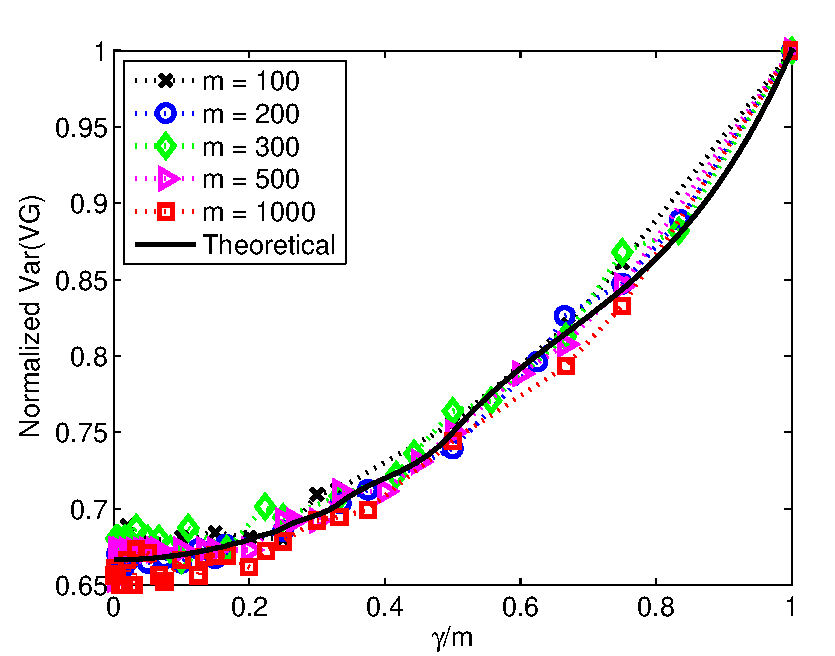
\includegraphics[width=.5\textwidth]{images/nv_varvar_discrete}}
	\subfloat[][CEP1]{
	   \label{fig:cep1_varvar}
	   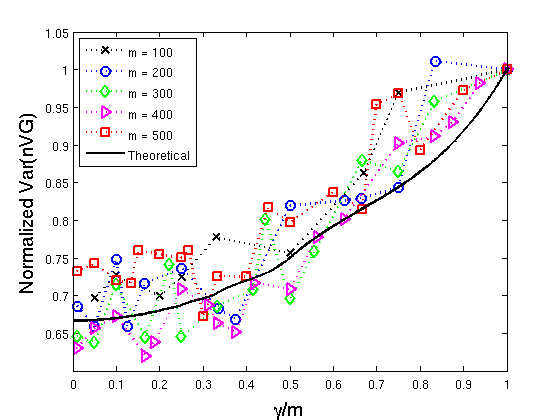
\includegraphics[width=.5\textwidth]{images/cep1_varvar}}
	\\
	\subfloat[][10D]{
	   \label{fig:10d_varvar}
	   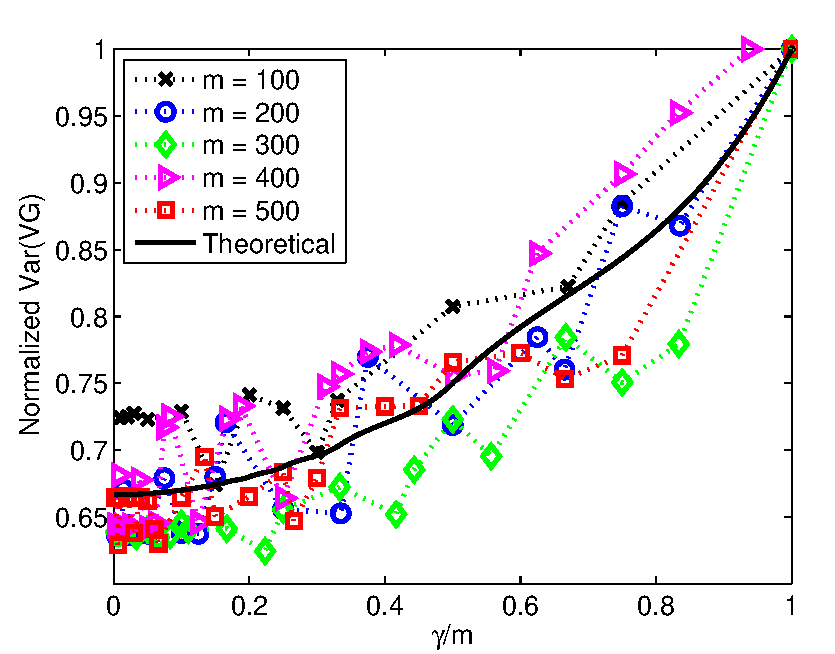
\includegraphics[width=.5\textwidth]{images/10D_varvar}}
	\subfloat[][DB1]{
	   \label{fig:db1_varvar}
	   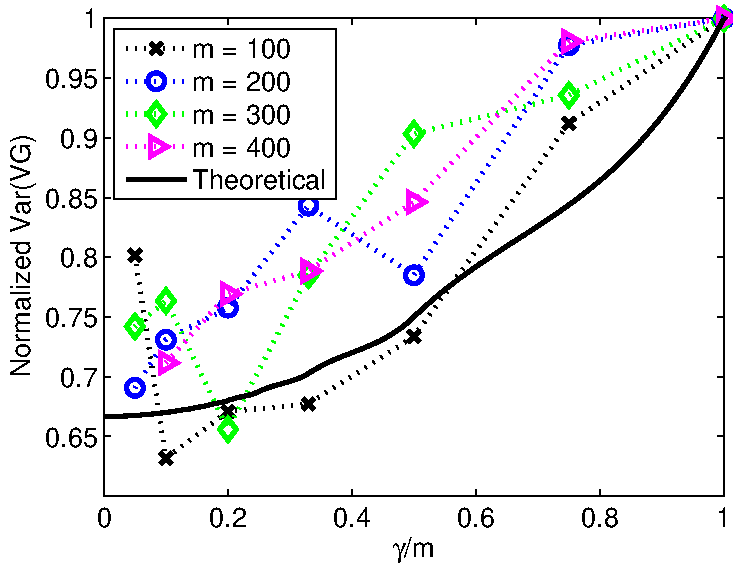
\includegraphics[width=.5\textwidth]{images/db1_varvar}}
	\caption{
		$\var{n VG}$ relative to the nonoverlapping counterpart across various values of $\gamma/m$ ($\gamma/m=1$ denotes the case of nonoverlapping batches) for test problems
		(a) NVD,
		(b) CEP1,
		(c) 10D, and
		(d) DB1
	}
\label{fig:varvar1}
\end{figure}


\begin{figure}[htb!]
	\centering
	\subfloat[][Expected Variance]{
	   \label{fig:nv_avgvar}
	   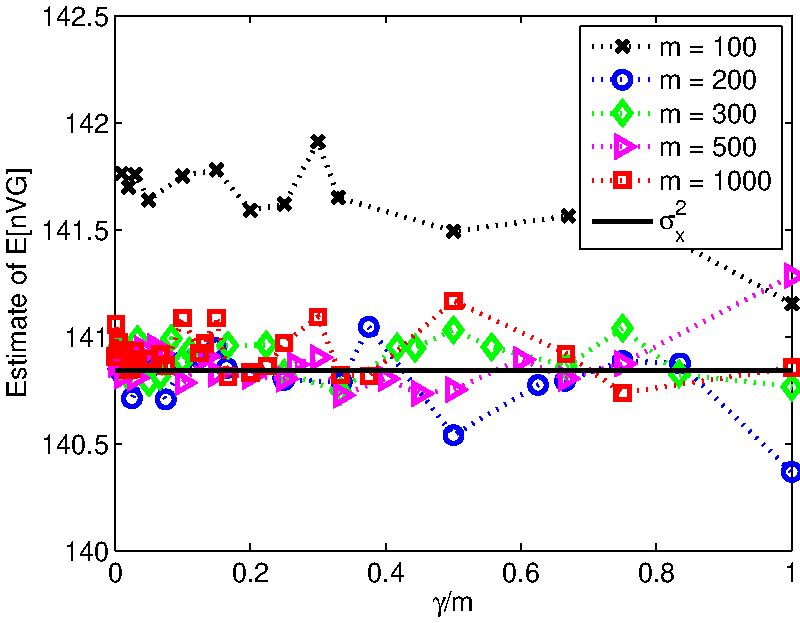
\includegraphics[width=.5\textwidth]{images/nv_avgvar_discrete}}
	\subfloat[][Coverage Probability]{
	   \label{fig:nv_cover}
	   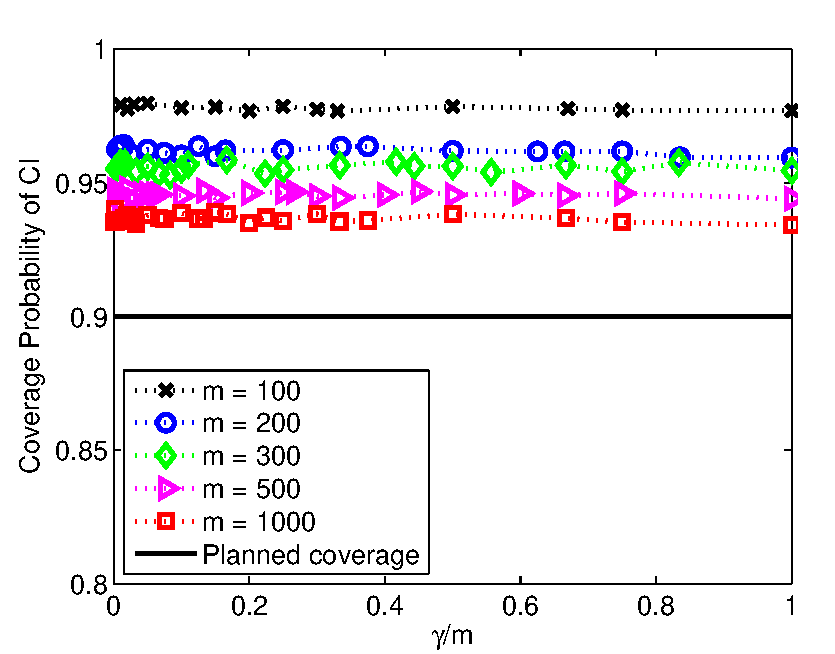
\includegraphics[width=.5\textwidth]{images/nv_cover_discrete}}
	\caption{ 
		Estimates of
		(a) $\e{nVG}$ and 
		(b) coverage probability of the CIs for various values of $\gamma/m$ ($\gamma/m=1$ denotes the case of nonoverlapping batches)
		 for NVD
	}
\label{fig:nv}
\end{figure}


Figure~\ref{fig:nv}(a) shows estimates of $\e{nVG}$ in the newsvendor problem for changing batch size and degree of overlap. 
We see that the expectation of the variance estimator does not change with increasing overlap. 
Although the estimate of $\e{nVG}$ looks large for $m=100$, the error from $\sigma^2_\xh$ is never more than 1\%.  
Estimates for $\e{nVG}$ showed a similar pattern for CEP1, 10D, and DB1.  
Those graphs are omitted for brevity.

Finally, Figure~\ref{fig:nv}(b) shows the coverage probability of CIs generated by OMRP for several values of $m$ across varying values of $\gamma/m$ for the newsvendor problem.  
The results of the overlapping batches estimators from the simulation literature show that coverage probability does not change with the degree of overlap, which we can  empirically see in this figure for OMRP for NVD.
We observed the same for CEP1, 10D, and DB1.  
The coverage probabilities from applying the (nonoverlapping) MRP algorithm to these problems presented in \cite{Bayraksan2006} agree with our results: for the newsvendor problem, coverage probability drops as $m$ increases and the coverage probability of CEP1 (not shown for brevity) remains fairly constant around the desired value of $90\%$. 
Coverage probability for 10D (not shown) and {\it estimated} coverage probability for DB1 (also not shown) were very high, more than $0.99$.  
The bias from solving (\ref{eq:sto_prog_m}) for these problems seems to be much more significant than the variance.

%%%%%%%%%%%%%%%%%%%%%%%%%%%%%%%%%%%%%
\subsection{Computational Efficiency}
\label{ssec:compeff}


The increased computational workload from applying overlapping batches to assessing solution quality raises the question of computational efficiency to estimate $VG$ in this context.
Computational efficiency can be defined as $[T(\gammab)\var{VG}]^{-1}$, where $T(\gammab)$ is the computation time spent to generate $VG$ for a given value of $\gammab$.
Because the variance of the overlapping variance estimator relative to the nonoverlapping (MRP) variant is known from (\ref{eq:var_reduct_formula}), we need only examine the computation time, which can be decomposed as $T(\gammab) = t(\gammab)\left(\nb\right)$. 
Here, $t(\gammab)$ is the average computation time per batch, which is multiplied by the number of batches.
Warm starting an algorithm may be used to decrease the computation time per batch for $\gammab < 1$, leading to a possible increase in computational efficiency. 

To investigate computational efficiency, we assumed that computation time per batch can be approximated as $t(\gammab) \propto \gammab^p$ for some $p \geq 0$.
The results for various values of $p$ are shown in Figure \ref{fig:efficiency}(a). 
This figure is constructed using $m = 1,000$, but the results do not change substantially with different values of $m$.
The graph is also scaled so that nonoverlapping batches produces a computational efficiency of 1. 
Efficiency gains increase with larger exponent $p$ but are positive even for small values of $p$ when $\gammab$ is sufficiently close to 1.
At $p=1$, i.e., for problems where computation time is proportional to the number of samples replaced in the batch, computational efficiency is maximized with maximally overlapping batches.
When $p=0.9$, computational efficiency is maximized at around $\gammab=0.3$.
When $p$ is $0.71$, on the other hand, computational efficiency is observed for values of $\gammab$ ranging from slightly lower than $0.3$ to $1$, and efficiency is maximized at a relatively flat region between $\gammab=0.5$ and $\gammab=0.8$.


\begin{figure}[thb!]
	\centering
	\subfloat[][Theoretical]{
	   \label{fig:efficiency_theory}
	   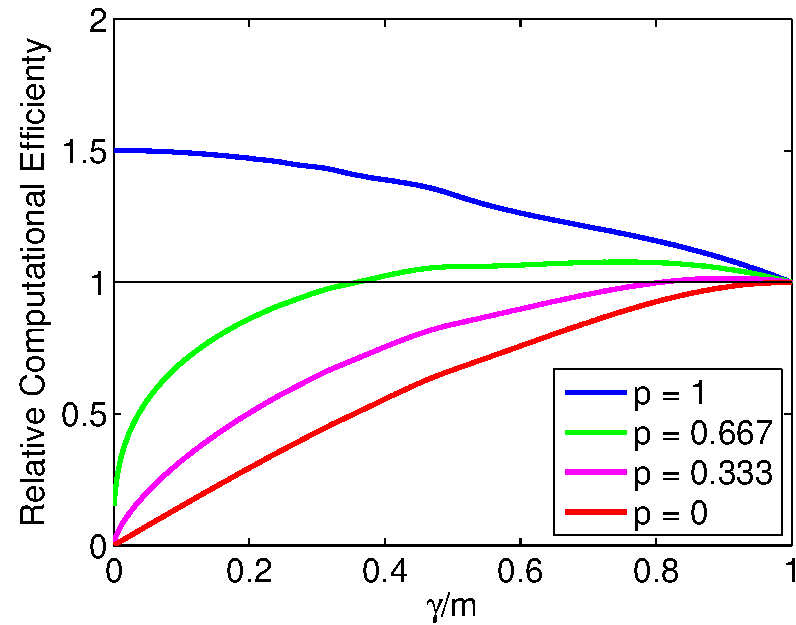
\includegraphics[width=.49\textwidth]{images/comp_efficiency_theory}}
	\subfloat[][Empirical for NVD]{
	   \label{fig:efficiency_nv}
	   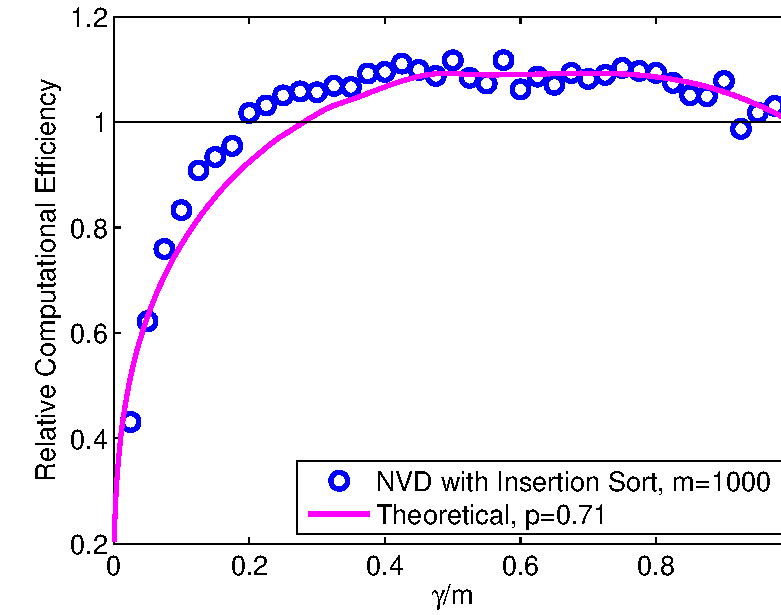
\includegraphics[width=.51\textwidth]{images/nv_comp_efficiency}}
		\caption{
		Computational efficiency of the OMRP variance estimator relative to the (nonoverlapping) MRP variance estimator measured
		(a) theoretically and
		(b) empirically for NVD using insertion sort
		}
\label{fig:efficiency}
\end{figure}


We tested this theoretical relationship using the newsvendor problem solved with insertion sort.
Insertion sort is an efficient algorithm when the values are already largely sorted. 
Therefore, as overlapping increases, insertion sort results in a decreased solution time per batch for the NVD problem. 
To test computational efficiency, we used $m = 1,000$ with $10,000$ runs.
The average computation time per batch was found empirically to be well approximated ($R^2 = 0.994$) by the power law with $p = 0.71$.
The empirically measured computational efficiency is compared to the theoretical result in Figure \ref{fig:efficiency}(b), where the theoretical computational efficiency, shown by a solid line, is repeated from Figure \ref{fig:efficiency}(a).
It appears that the empirical observations match the theoretical efficiency calculations well. 


A related question on computational efficiency asks whether OMRP is more efficient than nonoverlapping MRP with a larger number of batches.
When generating observations is cheap, one could alternatively increase the number of batches in MRP to obtain estimators with lower variances. 
In the nonoverlapping case, $\var{VG} \propto \frac{1}{k}$; so, decreasing $\var{VG}$ to the level of maximally overlapping batches requires a $50\%$ increase in the number of batches, and thus a $50\%$ increase in computation time.
Continuing on in this way for various values of $\gammab$, we obtain the solid black curve in Figure \ref{fig:comp_work_comparison}. 
This curve shows the increased computational effort for MRP because of an increased number of batches to obtain the same variance as OMRP across $\gammab$.
If the work increase by OMRP is less than this solid black curve, then OMRP is computationally more efficient than increasing the number of batches in MRP. 
Again, assuming average computation time per batch can be represented as $T(\gammab) \propto \gammab^p$, Figure \ref{fig:comp_work_comparison}(a) compares the increase in computational work for OMRP for several values of $p$ to the work increase for MRP to get an equivalent decrease in variance.
We again see that OMRP is advantageous for larger values of $p$.
For small values of $p$, some efficiency gain is observed at $\gammab$ values close to 1.
We tested this assertion empirically on NVD using insertion sort with $m=1,000$, taking an average of $10,000$ independent runs. 
The results, shown in Figure \ref{fig:comp_work_comparison}(b), appear to match the theory well. 


\begin{figure}[htb!]
	\centering
	\subfloat[][Theoretical]{
	   \label{fig:comp_work_comparison_theory}
	   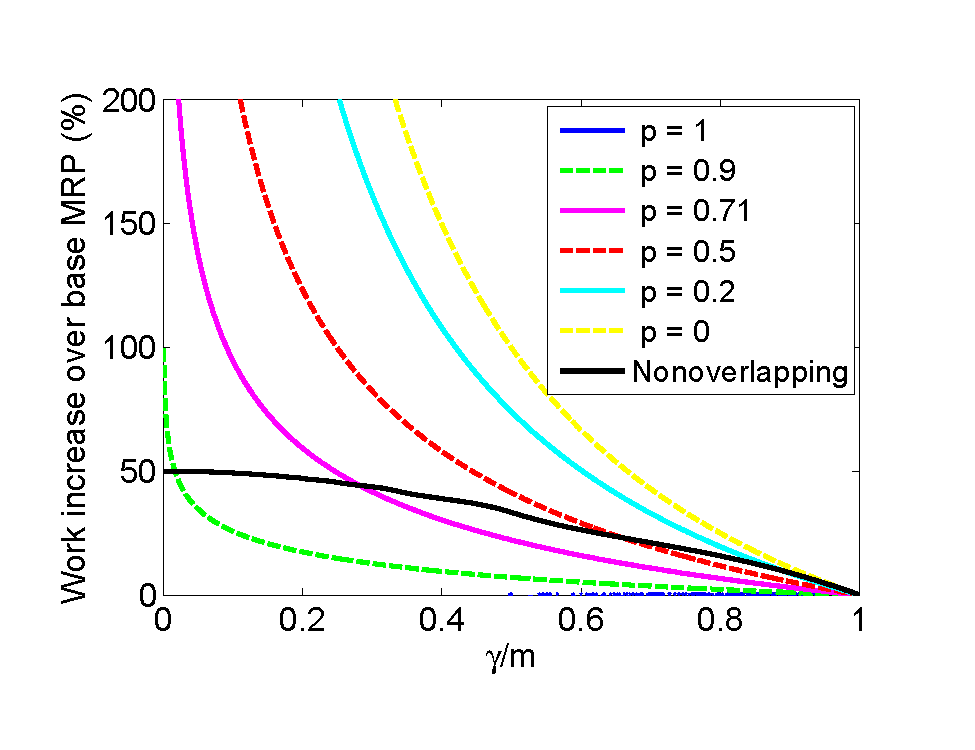
\includegraphics[width=.51\textwidth]{images/work_comparison}}
	\subfloat[][Empirical for NVD]{
	   \label{fig:comp_work_comparison_nv}
	   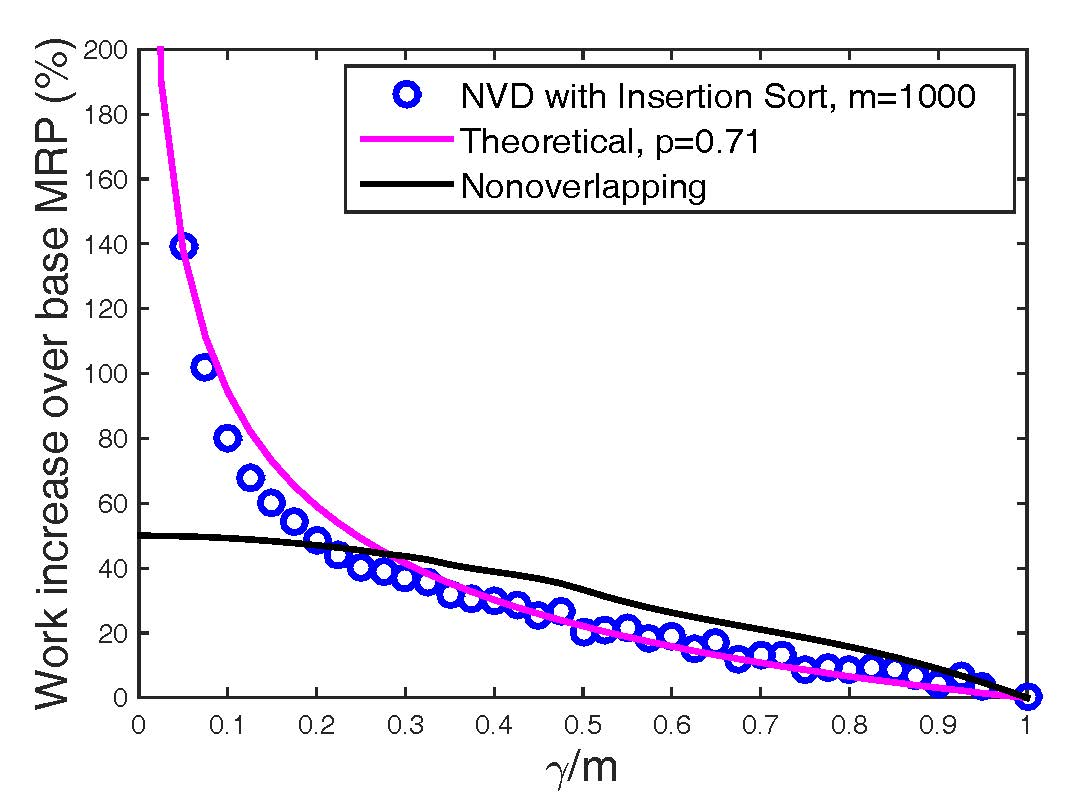
\includegraphics[width=.48\textwidth]{images/nv_work_comparison2}}
		\caption{
		Comparison of computational work required to obtain equivalent variance between the MRP variance estimator with increased number of batches and the OMRP variance estimator measured
		(a) theoretically and 
		(b) empirically for NVD using insertion sort
		}
\label{fig:comp_work_comparison}
\end{figure}


In cases where the exponent $p$ can be estimated, the above theoretical method may be used to determine a reasonable value for $\gammab$.
We recommend that users perform preliminary computations to determine how computation time per batch changes as $\gammab$ changes when warm starting is available. 
We can see in Figure \ref{fig:efficiency} that for some values of $p$, the efficiency gain is nearly flat over a region of $\gammab$.
In this case, we recommend choosing $\gammab$ near the right side of this region.
This choice keeps efficiency high while decreasing computation time and preventing large decreases in efficiency in the event that $p$ was overestimated.
For example, in the case of NVD, we recommend the use of $\gammab=0.8$ 
because this value provides minimal overall computation time across all values of $\gammab$ with the highest efficiency level for this problem.  
For situations where $p > 0$ but its size cannot be readily measured or estimated, we recommend selecting a large value of $\gammab$ such as $0.9$.
This allows for some increase in efficiency while remaining robust in the event that $p$ is smaller than expected.


%%%%%%%%%%%%%%%%%%%%%%%%%%%%%%%%%%%%%%%%%%%%%%%%%%%%%%%%%%%%%%%%%%%%%%%%%%%%%%%
\section{Conclusions}
\label{sec:concl}

We have applied the overlapping batch means method from simulation output analysis \citep{Meketon1984,Song1992,Welch1987} to the problem of assessing solution quality in stochastic programming, in particular, to Monte Carlo simulation-based estimators of optimality gaps \citep{Mak1999}. 
We have provided conditions under which (i) the resulting point estimator of the optimality gap and its associated variance estimator are consistent, (ii) OMRP variance estimators achieve asymptotically lower variances relative to the MRP variance estimator, and (iii) OMRP CIs are asymptotically valid. 
Empirical results indicate that asymptotic reductions in variance of the variance estimator show a similar decrease in OMRP at small sample sizes, while bias and coverage probability remain unaffected. 

Overlapping may increase the computational burden in the stochastic optimization setting.
By jointly considering computation time and variance, we have examined the computational efficiency of OMRP, and we have empirically demonstrated  efficiency by solving a newsvendor problem using insertion sort.
Our analysis illustrates that when warm starting is effective, computational efficiency gains can be observed across a wide range of overlapping degrees.
Even when warm starting is less effective, efficiency slightly increases for low degrees of overlap. 
Maximizing efficiency and then minimizing total computation time, we recommend  selecting the lowest degree of overlap across all the degrees with the highest efficiency for a given problem and solution method (with warm starting). 

Overall, the results in this paper suggest that OMRP could be an efficient method to estimate optimality gaps for a class of stochastic programs when warm starting is available and/or generating the observations is costly.
 

%%%%%%%%%%%%%%%%%%%%%%%%%%%%%%%%%%%%%%%%%%%%%%%%%%%%%%%%%%%%%%%%%%%%%%%%%%%%%%%
\section*{Acknowledgments}
The authors thank Andrzej Ruszczy{\'{n}}ski and Artur {\'{S}}wietanowski for
access to their regularized decomposition code, which was used to solve CEP1 and DB1. 
The authors are grateful to the associate editor and two anonymous referees for valuable suggestions that significantly improved both the content and the presentation of the paper. 
This research has been supported in part by the National Science Foundation under Grants DMS-0602173 and CMMI-1345626.


%%%%%%%%%%%%%%%%%%%%%%%%%%%%%%%%%%%%%%%%%%%%%%%%%%%%%%%%%%%%%%%%%%%%%%%%%%%%%%%
\bibliographystyle{abbrvnat}
\bibliography{omrp}
%%%%%%%%%%%%%%%%%%%%%%%%%%%%%%%%%%%%%%%%%%%%%%%%%%%%%%%%%%%%%%%%%%%%%%%%%%%%%%%

\end{document}
